\chapter{Heightmap}

% A few lines about heightmaps

The terrain itself in our demo is generated from a heightmap and is a
continuating on the work that we did in the first quarter (which
itself was based on earlier work). How a heightmap is loaded from a
texture and converted to geometry is pretty straight forward, and thus
won't be our focus here. Instead we will focus on our lighting model
and how it was derived from the generel lightmodel presented in
Real-time Rendering. We will talk about how we give the illusion of
more detailed geometry by implementing bump maps, which requires us
move the bumped normal in tangent space. Finally we will explain how
texture arrays where used to cut back on texture unit usage and
texture lookups when rendering.\\

% Geomorphing because it is in the vertex shader

However before we start on all the cool visuel effect, we must briefly
touch upon the subject of geomorphing to understand part of what is
going on in the vertex shader.\\

% Geomorphing removes terrain popping

The heightmap uses clustered level of detail, CLOD, to minimize vertex
processing overhead. An example can be seen in
\reffig{fig:tesselation} where a mound is rendered with three
different levels of detail, LOD. Vertex popping will occur when
switching between the different levels of detail, as the geometry is
suddenly deformed. Geomorphing can be used to remove this popping by
gently morphing in the new vertices. The technique is rather
simple. Instead of letting a verte pop into it's actual position when
changing LOD, the vertex is created between on the line between it's
to existing neighbours and then morphed into its actual
position. Because our terrain is a heightmap, geomorphing only needs
to be done along the y-axis.

\begin{figure}
  \label{fig:tesselation}
  \centering
  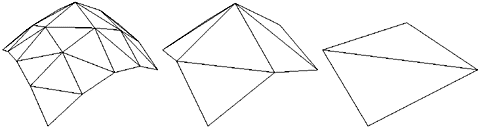
\includegraphics[width=5cm]{tesselation}
  \caption{A wireframe mound rendered with 3 different levels of detail.}
\end{figure}

% TODO Reference Geomorphing article

% We remove normal popping by using a normal map

Vertex popping has now been removed, but all other vertex attributes
must be morphed aswell to remove texture popping og normal
popping. Our heightmap texture coordinates are proportional to the
vertex positions so special attention needs to be taken to them. But
the normals will cause popping in the lighting. We could fix this by
morphing the normals, but instead we've used a normalmap to store the
normals in and retain our shading, even when the geometric detail is
reduced.

We assume that the terrain is not rotated, scaled or translated, so
all our vertices and normals are given directly in world/model
space. This is done to simplify some of our calculations and save a
normal transformation in the fragment shader.

\section{Lighting}

Because we're using shaders for rendering the heightmap, we need to
implement our own lighting effects. Since we're outside and rendering
natural environment our only lightsource is the sun, which is a
directional light. This allows us to ignore several aspects of the
lighting equation for one light source, equation 4.19 in Real-time
Rendering. 

\begin{displaymath}
  \mathbf{i}_{tot} = \mathbf{a}_{glob} \otimes \mathbf{m}_{amb} +
  \mathbf{m}_{emi} + c_{spot}(\mathbf{i}_{amb} + d(\mathbf{i}_{diff} + \mathbf{i}_{spec}))
\end{displaymath}

First of since we only have one lightsource in our entire
scene, the global ambience can be taken into account in the
lightsource's ambience, removing that expression from the
equation.

\begin{displaymath}
  \mathbf{i}_{tot} = \mathbf{m}_{emi} + c_{spot}(\mathbf{i}_{amb} + d(\mathbf{i}_{diff} + \mathbf{i}_{spec}))
\end{displaymath}

Also our lightsource is a directional light, so the spotlight factor,
$c_{spot}$, and attenuation, $d$, can safely be removed.

\begin{displaymath}
  \mathbf{i}_{tot} = \mathbf{m}_{emi} + \mathbf{i}_{amb} + \mathbf{i}_{diff} + \mathbf{i}_{spec}
\end{displaymath}

Lastly our emission factor is 0, so we end up with

\begin{displaymath}
  \begin{array}{rl}
    \mathbf{i}_{tot} &= \mathbf{i}_{amb} + \mathbf{i}_{diff} +
    \mathbf{i}_{spec}\\
    &= \mathbf{m}_{amb} \otimes \mathbf{s}_{amb} + (\mathbf{n} \cdot
    \mathbf{l}) \mathbf{m}_{diff} \otimes \mathbf{s}_{diff} +
    (\mathbf{v} \cdot \mathbf{r})^{m_{shi}} \mathbf{m}_{spec} \otimes
    \mathbf{s}_{spec} 
  \end{array}
\end{displaymath}

where we have used the following three formulas for ambient, diffuse
and specular lighting.

\begin{displaymath}
  \mathbf{i}_{amb} = \mathbf{m}_{amb} \otimes \mathbf{s}_{amb} 
\end{displaymath}

\begin{displaymath}
  \mathbf{i}_{diff} = (\mathbf{n} \cdot \mathbf{l}) \mathbf{m}_{diff} \otimes \mathbf{s}_{diff} 
\end{displaymath}

\begin{displaymath}
  \mathbf{i}_{spec} = (\mathbf{v} \cdot \mathbf{r})^{m_{shi}} \mathbf{m}_{spec} \otimes \mathbf{s}_{spec} 
\end{displaymath}

where $\mathbf{n}$ is the surface normal, $\mathbf{l}$ is the
direction of the light, $\mathbf{v}$ is the vector pointing from the
camera to the surface point and $\mathbf{r}$ is the reflection of the
light around the normal. All the vectors are assummed to be normalized
and can be seen on \reffig{fig:lightVectors}.

\begin{figure}
  \centering
  \label{fig:lightVectors}
  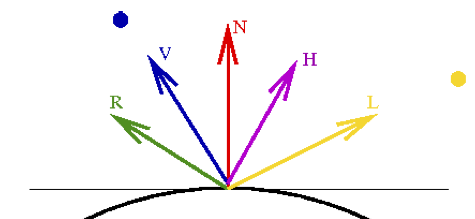
\includegraphics[width=5cm]{lightVectors}
  \caption{The vectors used in lighting calculations}
\end{figure}

% @TODO add images

\begin{figure}
  \label{fig:lightComponents}
  \centering
  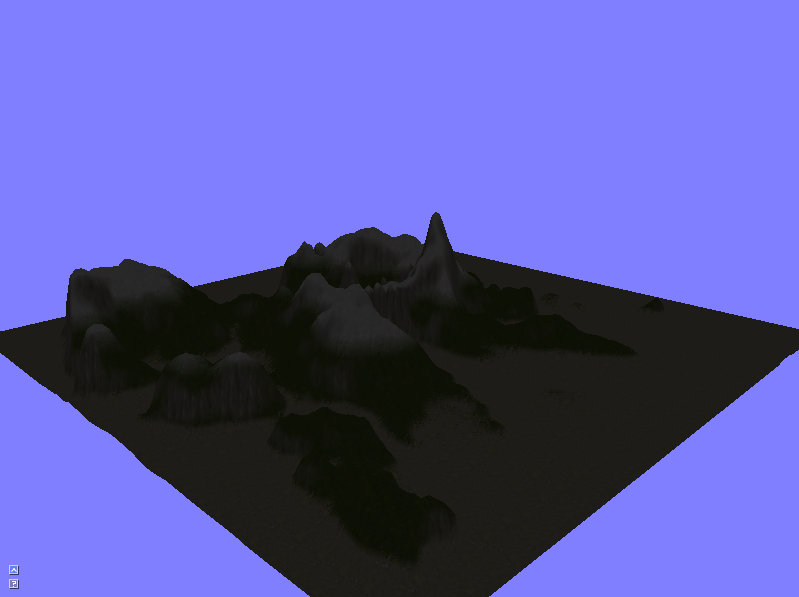
\includegraphics[width=5cm]{ambient}
  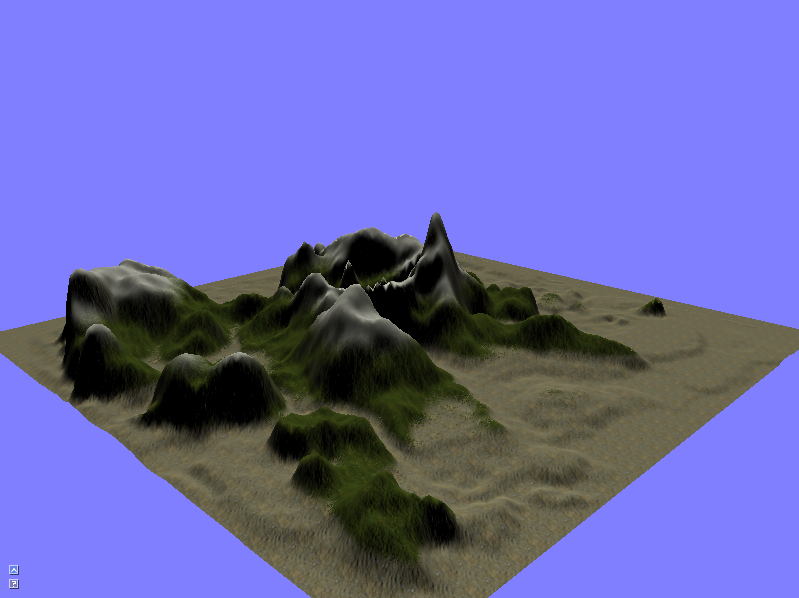
\includegraphics[width=5cm]{diffuse}
  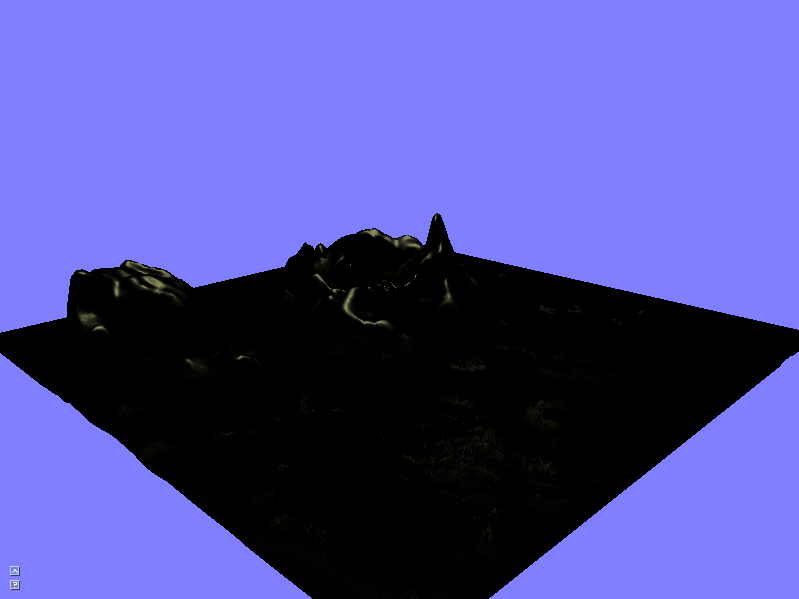
\includegraphics[width=5cm]{specular}
  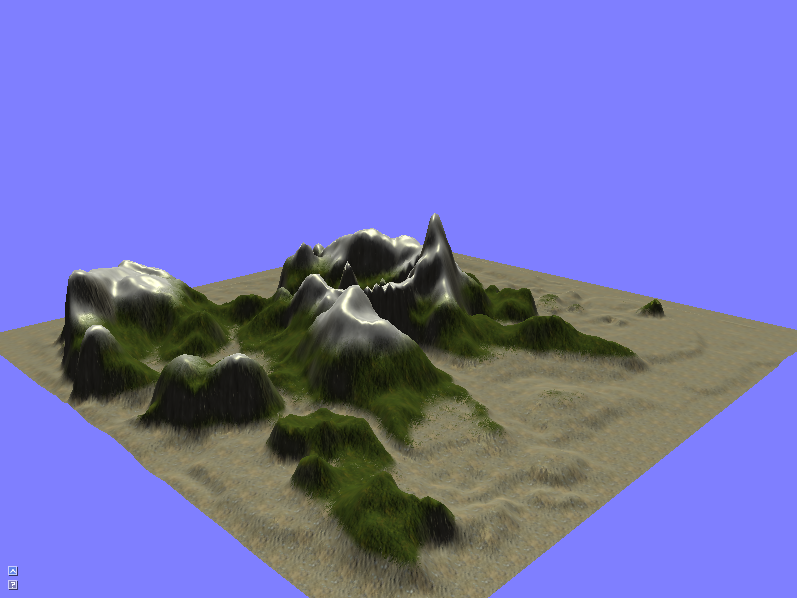
\includegraphics[width=5cm]{lightSum}
  \caption{Images of the different light components making up the terrain lighting.}
\end{figure}


The contribution of each factor to the final image can be seen in
\reffig{fig:lightComponents}.

Now if we restrict our material to only specify one color instead of a
seperat color for ambient, diffuse and specular, we can reduce the
equation to 

\begin{displaymath}
  \begin{array}{rl}
    \mathbf{i}_{tot} &= \mathbf{m}_{color} \otimes \mathbf{s}_{amb} + (\mathbf{n} \cdot
    \mathbf{l}) \mathbf{m}_{color} \otimes \mathbf{s}_{diff} +
    (\mathbf{v} \cdot \mathbf{r})^{m_{shi}} \mathbf{m}_{color} \otimes
    \mathbf{s}_{spec} \\
    &= \mathbf{m}_{color} \otimes (\mathbf{s}_{amb} + (\mathbf{n} \cdot
    \mathbf{l}) \mathbf{s}_{diff} + (\mathbf{v} \cdot
    \mathbf{r})^{m_{shi}} \mathbf{s}_{spec}) \\
  \end{array}
\end{displaymath}

This restriction is more physically correct, in the sense that only
the color of the material is now shaded with respect to the different
light components, but is also more restrictive to artists.\\

In the above formulas the specular lighting has been given by the
Phong lighting equation, $\mathbf{i}_{spec} = (\mathbf{v} \cdot
\mathbf{r})^{m_{shi}} \mathbf{m}_{spec} \otimes \mathbf{s}_{spec}$,
where $\mathbf{m}_{spec} = \mathbf{m}_{color}$ and $\mathbf{r} = 2
(\mathbf{n} \cdot \ \mathbf{l}) - \mathbf{l}$.

A faster approximation was proposed by Blinn. Instead of basing the
specular highlight on the angle between the view direction and
reflection vector, He proposed to base it on the angle between the
halfvector, a vector halfway between the view vector and light vector
given by $\mathbf{h} = (\mathbf{l} + \mathbf{v}) / \|\mathbf{l} +
\mathbf{v}\|$, and the normal. An approximate relationship between the
two is given in Real-time Rendering as

\begin{displaymath}
  (\mathbf{r} \cdot \mathbf{v})^{m_{shi}} \approx (\mathbf{n} \cdot \mathbf{h})^{4m_{shi}} 
\end{displaymath}

Both specular light models have been implemented in the terrain
fragment shader and the results can be seen in \reffig{fig:specularLight}

\begin{figure}
  \label{fig:specularLight}
  \centering
  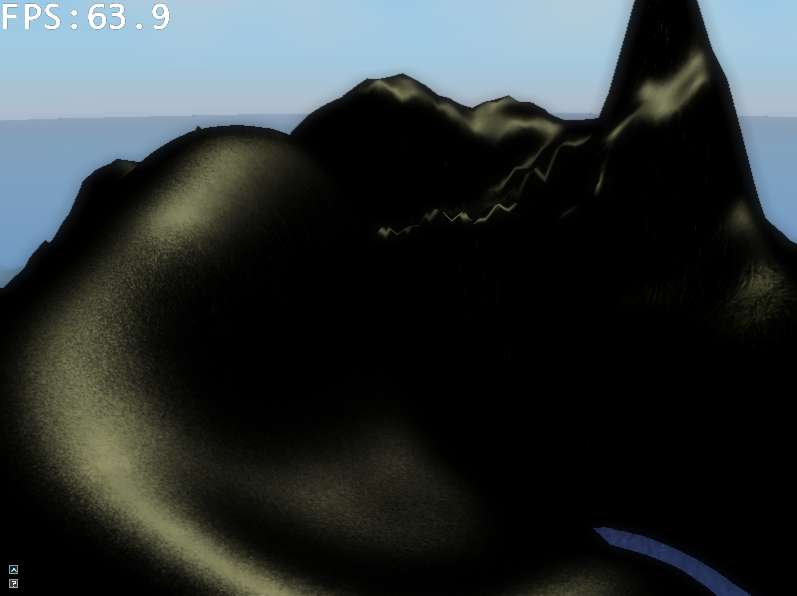
\includegraphics[width=5cm]{phongSpec}
  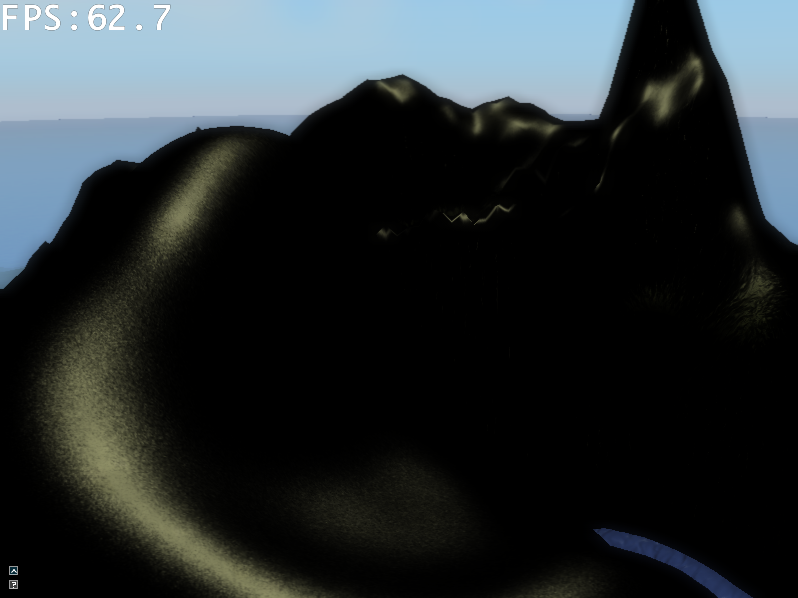
\includegraphics[width=5cm]{blinnSpec}
  \caption{A comparison of Phong specular lighting and Blinn specular lighting. The image on the left is Phong and the right is Blinn.}
\end{figure}


\section{Bump mapping}

With the terrain shaded by the sun, it's time to improve on the detail
of the lighting by adding 'bumps' to the surface, or more precisely
manipulating the normal to create a bumpy feel. We do this by storing
the normals of a surface in a texture, then instead of using the
interpolated geometric normal for light calculations, we transform the
texture normal into tangent space and use that for lighting.

In order to do that we need the interpolated normal, tangent and
bitangent as the axes of our tangent space coordinate system. Since
we're using the y-axis as up, the normal will be our y-axis in the
tangent space coordinate system. The tangent and bitangent are
normalized vectors perpendicular to the normal and lie along the bump
maps texture coordinate axes. Normally calculating them is done as a
preprocess and they are stored as vertex attributes or in our case a
tangent- and bitangentmap. However due to the heightmap being a 2D
array of vertices with texture coordinates proportinal to the x- and
z-coordinates, we can calculate the tangents directly in the
shader. This saves us 2 texture lookup and the need to bind additional
textures.

Since our texture coordinates are axis-aligned, the tangent will lie
in the xy-plane and the bitangent is placed in the yz-plane. Here we
will focus on calculating the tangent, but the same principle can be
applied to calculate the bitangent.

The interpolated normal is our approximation of a vector perpendicular
to the terrain surface. It can therefore also be used to calculate
vectors along that surface, specifically the tangent along the
xy-plane. This can be done by taking the cross product between the
normal, $n$, and the unit vector along the z-axis, $z_i = (0,0,1)$, which
will ensure that the tangent is both perpendicular to the normal, ie.
lying in the plane, and perpendicular to the z-axis, which places it
in the xy-plane. The calculations are

\begin{displaymath}
  \begin{array}{rl}
  n \times z_i &= (n_x, n_y, n_z) \times (0,0,1)\\
  &= (n_y 1 - n_z 0, n_z 0 - n_x 1, n_1 0 - n_2 0) \\
  &= (n_y, - n_x, 0) \\
  \end{array}
\end{displaymath}

which is the direction of the tangent. All that is left is to
normalize the vector to get the tangent.

The tangent, bitangent and normal now make up the axes in tangent
space and can be used to either move the direction of the light from
global space to tangent space or move the bumped normal from tangent
space to global space. For this project the latter was chosen to
easier incorperate the shaders into a deferred lighting pipeline in
the future.

The glsl code can be seen here

%TODO reference code in appendix or here

\section{Ground layers}

Several layers of ground textures have been added to the heightmap for
a more diverse terrain. There is a sand layer, a grass layer and a
snow layer. Rocks have also been added where slopes are steep enough,
but the focus is on layered texturing.

% No blending between layers

For our layered textures we chose to use the GL\_EXT\_texture\_array
extension, which allows us to create an array of textures that are
mipmapped individually. Unfortunately the texture array does not blend
across the different layers, so this has to be handled by the fragment
shader.

% We could have used a 3d texture instead but then we would loose
% mipmapping and we want our mipmapping!

An alternative would be placing all the layers in a 3D texture, which
could then blend between the different layers upon texture lookup in
the shader. The downside to this is that using mipmapping on a 3D
texture, will 'blend' the different layers together, creating a
brownish looking texture in the second mipmap level and onwards. The
only solution to this would be to disable mipmapping, which results in
a performance penalty and creates flickering textures.

So in the end we opted for texture arrays over 3D textures and
implemented the blending ourselves.

For each layer several parameters can be chosen

\newcommand{\layerProp}[2]{\item \textbf{#1} - #2}
\begin{itemize}
  \layerProp{startHeight}{When the layer should start to blend in.}
  \layerProp{blending}{How many units of height it takes the layer to
    become completely opaque.}
  \layerProp{spec[i]}{The specular factor of the i'th layer, where the
    x-component specifies a specular intensity scalar and the
    y-component is the shininess}
\end{itemize}

How much of the i'th layer should be visible, $factor_i$ is then
trivially calculated by

\begin{displaymath}
  factor_i = (height - startHeight_i) / blending_i
\end{displaymath}

Since it doesn't make sense for a layer to be more than completely
transparent or opaque , ie. a factor of 0 or 1, we clamp the factor
between these values. The actual index of the layer to be used in the
texture array is then quite easy to calculate. We simply add all the
factors. 

And example could be layer 2 is completely opaque and layer 3 is 40\%
visible. At that height layer 1 will also think it should be
completely opaque. The layer height is then $1 + 1 + 0.4 = 2.4$, which
means that the base layer is 2 and that has be blended with 40\% of
the 3'rd layer.

% TODO ref appendix or show layer code

When specifying the height or the terrain a little randomness is added
to it from the normalmap. This is done to avoid smooth transitions
between the layers and give the terrain a more natural feel.

%\section{Vertex shader}

% Geomorphing, fordele/ulemper, alternativer

% Terrain skal placeres i worldspace, acceptabel antagelse og spare os
% for matrix multiplicationer.

%\section{Fragment shader}

% Light calculations (blinn/phong)

% Calculating the appropriate texture index and blending with the next
% layer.

% Normals and tangent space

% Bump mapping (rotating the normal in tangent space)

\section{Summary}




% Place future work here or after the conclusion?

% Clip mapping, will make it easy to use LOD shaders (out with bump
% and specular) Also simply geometry LOD using alpha blending (take
% care to render geometry in the correct order)

% Optimized texture lookup (saving 2 normals in 4 channels and
% blending them, not implemented)



%%% Local Variables:
%%% mode: latex
%%% TeX-master: t
%%% TeX-PDF-mode: t
%%% End:
